% https://tex.stackexchange.com/a/416431
\documentclass{beamer}

\usepackage{tikz}

\begin{document}

\begin{frame}

\begin{columns}[onlytextwidth]
    \begin{column}{.15\textwidth}
        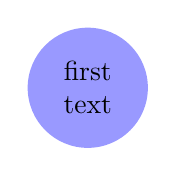
\begin{tikzpicture}
        \node[fill=blue!40!white,circle,text width=1cm,align=center] {first text};
        \end{tikzpicture}
        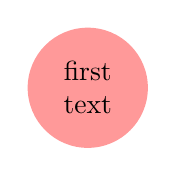
\begin{tikzpicture}
        \node[fill=red!40!white,circle,text width=1cm,align=center] {first text};
        \end{tikzpicture}       
        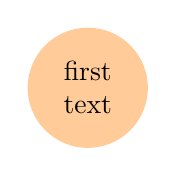
\begin{tikzpicture}
        \node[fill=orange!40!white,circle,text width=1cm,align=center] {first text};
        \end{tikzpicture}       
    \end{column}
    \begin{onlyenv}<1>
        \begin{column}{.2\textwidth}
            \includegraphics[width=\textwidth]{example-image-a}
        \end{column}
        \begin{column}{.6\textwidth}
            text 1
        \end{column}    
    \end{onlyenv}
    \begin{onlyenv}<2>
        \begin{column}{.2\textwidth}
            \includegraphics[width=\textwidth]{example-image-b}
        \end{column}
        \begin{column}{.6\textwidth}
            text 2
        \end{column}    
    \end{onlyenv}   
    \begin{onlyenv}<3>
        \begin{column}{.2\textwidth}
            \includegraphics[width=\textwidth]{example-image-c}
        \end{column}
        \begin{column}{.6\textwidth}
            text 3
        \end{column}    
    \end{onlyenv}
\end{columns}

\end{frame}

\end{document}
